\chapter{Introduction}
This dissertation concerns the work performed on the SIRIUS storage ring sextupole mangets with the objective to optimize the ring's Dynamic Aperture and injection efficiency. The text is organized as follows:
\begin{itemize}
    \item Chapter 1 introduces syncrhotron light sources and the SIRIUS project;
    \item Chapter 2 introduces the theoretical and scientific background on the dynamics of particles in accelerators. The chapter goal is to define the Dynamic Aperture;
    \item Chapter 3 introduces and justifies online optimization in accelerators and the Robust Conjugate Direction Search (RCDS) algorithm;
    \item Chapter 4 describes the experimental methods and setup for the online optmization experiments and the results achieved;
    \item Chapter 5 concludes this dissertation presenting the final remarks.
\end{itemize}

\section{Storage ring-based synchrotron light sources}
Synchrotron radiation (SR) is the electromagnetic radiation emitted by charged relativistic particles when accelerated perpendicularly to their motion. The phenomenon was theoretically predicted in the early 1900s when Liénard and Wiechert calculated the retarded potentials for point particles.

The first experimental observation of synchrotron light occurred at General Electric's $70~\unit{Mev}$ synchrotron accelerator, justifying the adoption of the term "synchrotron" in its name. Modern synchrotron light sources primarily rely on two particle acceleration technologies: free-electron lasers and storage rings. Here, we focus on storage ring-based synchrotron light source facilities.

In storage ring-based synchrotron light sources, ultra-relativistic electron beams are stored for extended periods within a chamber in ultra-high vacuum to produce synchrotron light. The beams are maintained in stable orbits by the fields of an array of magnets--the lattice--which provide both bending, focusing and trajectory-correction fields. The beam is also periodically influenced by radiofrequency cavities, which replenish the energy radiated away in the form of light.

The main figure of merit for the quality of a SR source is the \textit{brightness}, defined as the photon flux per unit area and per unit solid angle at the source:
\begin{equation}
    B(\omega) = \frac{F(\omega)}{\Omega_{xx^\prime}\Omega_{yy^\prime}\Delta \omega/\omega},
\end{equation}
where $F(\omega)$ is the photon flux at energy $E=\hbar\omega$, $\Omega_{uu^\prime}$ is the the $(u,u^\prime)$-plane photon phase-space volume and $\Delta\omega/\omega$ is the frquency bandwith, which is typically about $0.1\%$. The photon phase space volume depends on the convolution of the electron beam distribution with the distribution of the photons emmited by a single electron. The latter depends on the photon energy and the emission process, while the former is related to the average electron beam phase-space volume: the emmitance, which depends on the magnetic lattice.
\todo[inline]{review the theory}

Synchrotron light sources can be classified based on their brightness/emmitances. The community initially interested in synchrotron radiation (SR) for imaging experiments obtained SR parasitically from high-energy and nuclear physics machines in the early 1960s, marking the era of first-generation synchrotron light sources. Typical emmitances were about X. The second-generation machines consist on those designed exclusively for SR production. They emerged in the 1980s and had emittances of the order of X.

The 1990s saw a growing demand for higher brightness, leading to the development of third-generation machines. These machines introduced insertion devices such as wigglers and undulators, significantly enhancing brightness by increasing radiative damping. Additionally, these devices allowed precise control over radiation energy and polarization.

The era of the fourth-generation of SR sources commenced with the MAX-IV machine in Lund, Sweden, in 2015. Fourth-generation machines achieved a notable reduction in emittance, thanks to recent technological advancements. Following MAX-IV, an upgrade of the ESRF facility and the launch of SIRIUS in Campinas marked significant milestones. SIRIUS is particularly noteworthy as the first of its generation in the global South.

\section{The SIRIUS project}
SIRIUS is a 4th generation storage ring-based synchrotron light source. It was designed, built, and is operated by the Brazilian Synchrotron Light Laboratory (LNLS), on the campus of the Center of Research in Energy and Materials (CNPEM), in Campinas, Brazil.

SIRIUS succeeded the first Synchrotron Light Source in Brazil, UVX, which opened to users in 1997 and served the community until the beginning of SIRIUS commissioning in August 2019 when it was shut down\footnote{The UVX project led to the creation of LNLS, which marked a new model for scientific research in Brazil, based on social organizations under contracts with the Ministry of Science Technology and Innovations. LNLS paved the way for national labs (NL), including labs on biosciences (LNBio), nanotechnology (LNNano), and bio-renewables (LNBR), which are also located at the CNPEM campus, along with many other NLs across Brazil}.

The SIRIUS project started in 2008 in response to the growing scientific demands of the synchrotron community. By 2012, it evolved into the project of a fourth-generation machine. Presently, SIRIUS stands as the most complex scientific infrastructure ever consturcted in Brazil, with the ambitious goal of positioning the country at the forefront of global leadership in synchrotron light sources. This state-of-the-art synchrotron was meticulously designed to shine as the brightest in its energy category, and has the capacity to host up to 40 beamlines. As of the time of this writing, SIRIUS holds the distinction of being the sole fourth-generation synchrotron radiation source in the southern hemisphere and one of merely three 4GSRs in operation across the globe.

SIRIUS finished commissioning in 2022 and since March 2023 is receiving its first external users. At the time of this writing, it has 6 operating beamlines, 4 beamlines in commissioning and 4 under construction and installation. It is currently operating for user's beam with a $100~\unit{mA}$ current, with frequent beam injections throughout the day, a scheme known as ``top-up'' mode. SIRIUS is expected to achieve $350~\unit{mA}$ current when the system of two superconducting radiofrequency cavities is installed.

\subsection{Storage ring-based light source subsystems}
Typical systems comprising a storage ring synchrotron light source facility include
\begin{itemize}
    \item an injection system: including the electrons source, beam transport lines, and the first accelerating systems: the linear accelerator and the booster ring, a circular accelerator. At SIRIUS, the linear accelerator provides the booster with a $150~\unit{MeV}$ beam. The booster further ramps the energy up to $3~\unit{GeV}$, which is the storage ring operation energy;
    \item storage ring: where ultra-relativistic electrons are kept stable for hours within the vaccum-chamber, oscillating about a closed orbit for the production of synchrotron light;
    \item beamlines: which steer the photon beams towards the experimental cabins whre the samples are placed for the experiments based on light-matter interaction, such as spectroscopy, crystallography, tomography and others.
\end{itemize}

Synchrotron storage rings store ultra-relativistic electron beams in proximity to a reference design orbit. This orbit is determined by the strengths of the deflection magnets, the dipoles, and the operation energy of the beams. A pure dipole provides an uniform and homogeneous magnetic field perpendicular to the floor. To define a closed orbit, the overall bending angle provided by the dipoles along the entire ring must equal $2\pi$ radians.

To maintain electrons in close proximity to the reference orbit, focusing is achieved through gradient fields, primarily generated by quadrupole magnets at SIRIUS. The strength of quadrupole fields increase linearly with deviations from the closed orbit, effectively acting as a spring force.

Focusing and deflection are energy-dependent, which means small deviations from the nominal operating energy can result in differential focusing. Drawing an analogy from geometric optics, the beam's focusing behavior at the "lens" (quadrupoles) depends on its "color" (energy). To correct for these chromatic aberrations, the use of "glasses" becomes necessary. In the context of accelerators, sextupole fields serve as these corrective lenses. They introduce geometric aberrations to counteract the chromatic ones, resulting in approximately uniform, energy-independent focusing.

\begin{figure}
    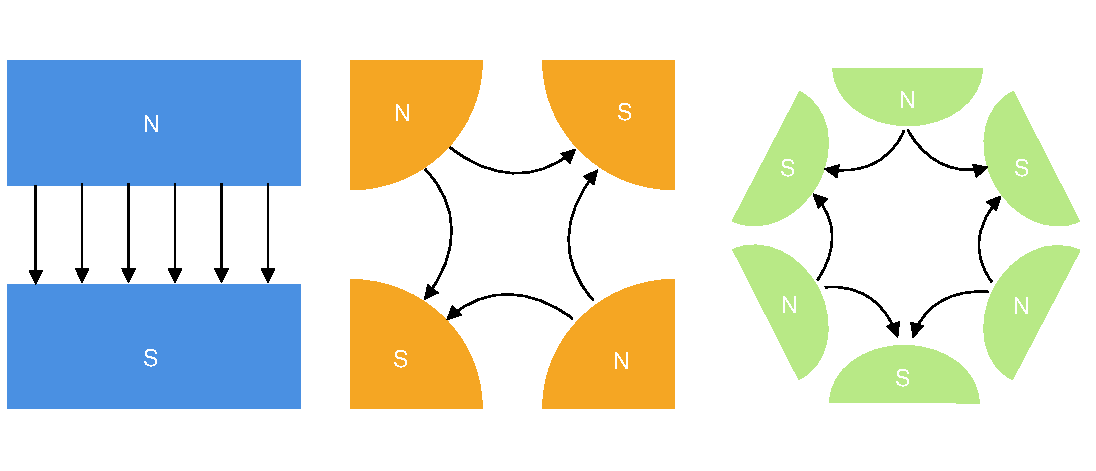
\includegraphics[width=\textwidth]{Images/magnets.pdf}
    \caption{Schematic representation of the magnets comprising SIRIUS lattice and their fields profile. From left to right: dipole magnet, quadrupole magnet and sextupole magnet.}
\end{figure}
\begin{figure}
    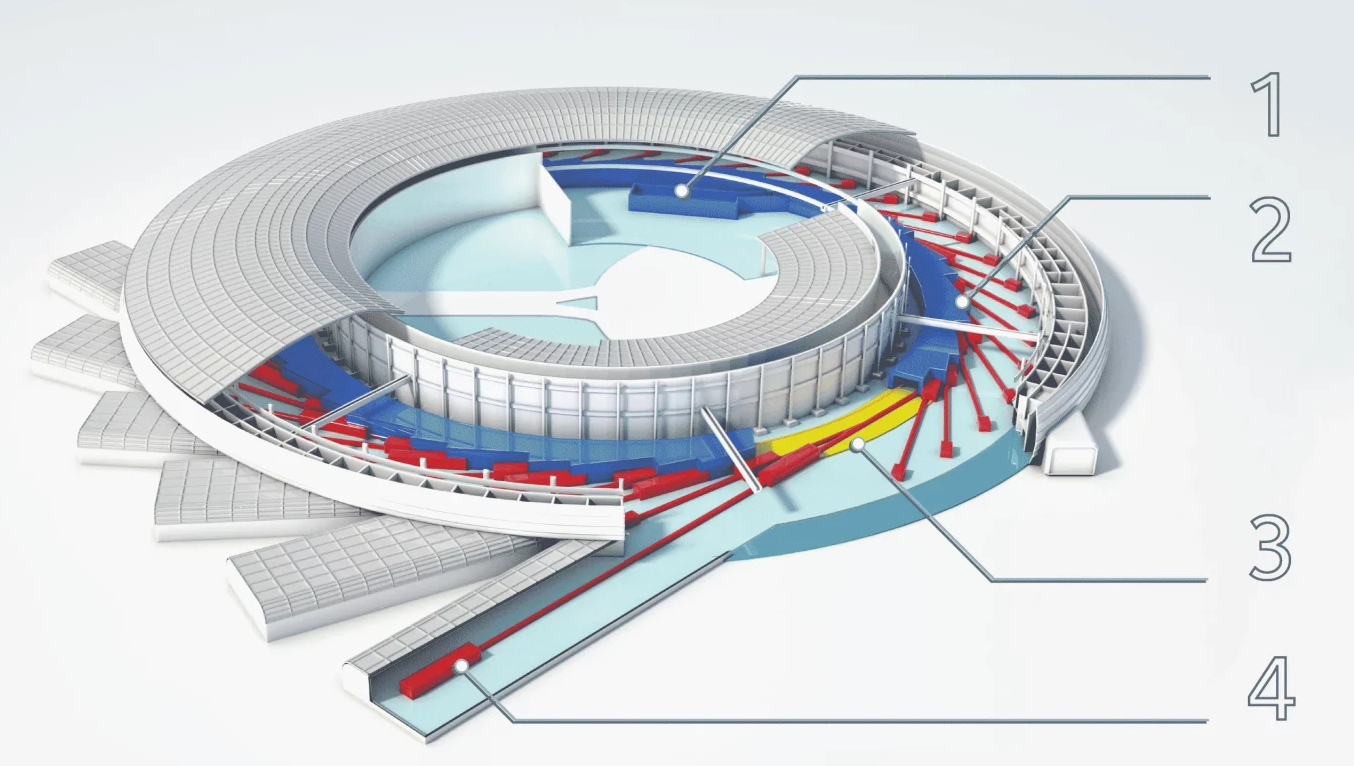
\includegraphics[width=\textwidth]{Images/sirius_facility.png}
    \caption{Schematic view of the SIRIUS installations. 1) Linear accelerator (LINAC); 2) Concrete tunnel housing the booster accelerator and the storage ring; 3) storage ring; 4) beamlines. From \href{https://lnls.cnpem.br/sirius/como-funciona-o-sirius/}{LNLS website}.}
\end{figure}
\section{This dissertation problem}
The pursuit of low emittances and high brightness has driven the accelerator community toward the fourth-generation of storage rings. Achieving such low emittances was possible because of series of technological advances which enabled the use of the multi-bend achromat (MBA) lattice. MBA lattices require intense gradient fields provided by quadrupole magnets, which, in turn, demands the presence of strong sextupolar fields to compensate for chromatic effects. Since sextupoles provide nonlinear fields, the dynamics in fourth-generation storage rings has become increasingly nonlinear.

A quasi-periodic nonlinear dynamics, when subjected to even the slightest perturbations—such as small field errors stemming from rotation, alignment, or fields excitation errors—can potentially become unstable at large oscillation amplitudes. These instabilities impose constraints on the maximum transverse oscillation amplitudes that the machine can accommodate. This specific amplitude below which motion stable is referred to as the Dynamic Aperture of the ring.

Under normal operating conditions, the equilibrium beam distribution is considerably smaller than the Dynamic Aperture (DA), and the dynamics can be well studied and analyzed using a linear approximation theory. However, there are specific scenarios where the DA becomes crucial for the operation, notably during the injection process.

During injection into the storage ring for beam accumulation, the beam is extracted from the booster accelerator and guided toward the storage ring through a transport line. Subsequently, it is deflected by pulsed nonlinear magnet to align it parallel to the storage ring tangent, albeit with a horizontal offset of approximately $x=-8~\unit{mm}$. If the DA is smaller than this offset, it imposes limitations on the injection efficiency.

The placement, symmetry, and strength of sextupoles magnets--the nonlinear lattice-- were determined through a multi-objective optimization process, primarily focusing on improving the simulated dynamic aperture and beam lifetime of the machine's computer model. This optimization work considered the average performance of the lattice configurations while accounting for various magnet errors that simulate the expected errors in the actual machine.

Several models, with several errors distribution among the magnets were generated, and the DA and lifetime for a given lattice configuration was calculated by simulating the electron beams motion for several turns (tracking simulations). The final figure of merit for a lattice consisted on the average DA and lifetime it provided to the ensemble of machines. The best-performing machine lattice found during this process was adopted as the nominal lattice which was subsequently implemented during the commissioning phase of the machine.

However, the operating machine consists on a practical realization of a specific error configuration, which defines the physically realized magnetic lattice and its overall performance. The best-performing lattice on average is not necessarily the optimum lattice for this errors realization.

Assuming the realized lattice closely approximates the optimum setup, i.e. that errors are small, it is reasonable to assume that making minor tweaks and adjustments to the strengths of the sextupoles can adapt the lattice to match the actual distribution of errors in the physical system. This fine-tuning process can result in improved nonlinear dynamics performance, expanding the Dynamic Aperture (DA), and ultimately enhancing both injection efficiency and its stability.

Online optimization consists on employing computer-automated search strategies to systematically explore various sextupole configurations with the goal of identifying the one that yields the largest dynamic aperture while not interfering in other machine parameters.

It is shown in this dissertation that this process can succesfully improve the dynamics performance. Prior to the optimization work, the Dynamic Aperture was measured to be \todo{get data}, which rendered an average of \todo{get data} injection efficiency. The main difficulty was the typycal fluctuations in the effciency \todo{get data}.
